\section{Approach} \label{sec:approach}

We aim to measuring the performance of TCP under different network topologies.
According to our motivation, we need to build topologies containing several
switches and each switch is linked with a number of hosts. For simplicity,
we formalize the topology as containing 7 switches and each switch has only 
one host connected. We choose the number 7 because a tree topology need 7 nodes
to build a symmetric tree structure. And for other topologies, \eg star topology
and line topology, 7 nodes can also build a symmetric structure. The switches are named
as s{\it x} and the corresponding hosts are named as h{\it x} where {\it x} $\in [0, 6]$.

The network topologies considered in this paper are presented in Figure~\ref{fig:topo}.
There are many types of network topologies in read world, but
due to some reasons we will discuss in Section~\ref{sec:discussion}, we only consider
3 of them in this paper: {\it Line}, {\it Tree} and {\it Star}. 

\begin{figure}[ht]
\centering
\subfloat[][Line Topology] {
	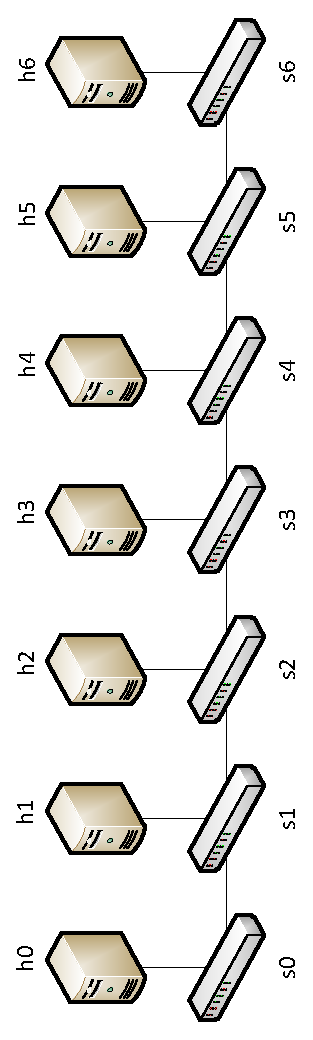
\includegraphics[angle=-90, width=0.45\textwidth, clip]{figs/line.eps}
}

%\subfloat[][Ring Topology] {
%	\includegraphics[angle=-90, width=0.30\textwidth, clip]{figs/ring.eps}
%}

\subfloat[][Star Topology] {
	\includegraphics[angle=-90, width=0.35\textwidth, clip]{figs/star.eps}
}

\subfloat[][Tree Topology] {
	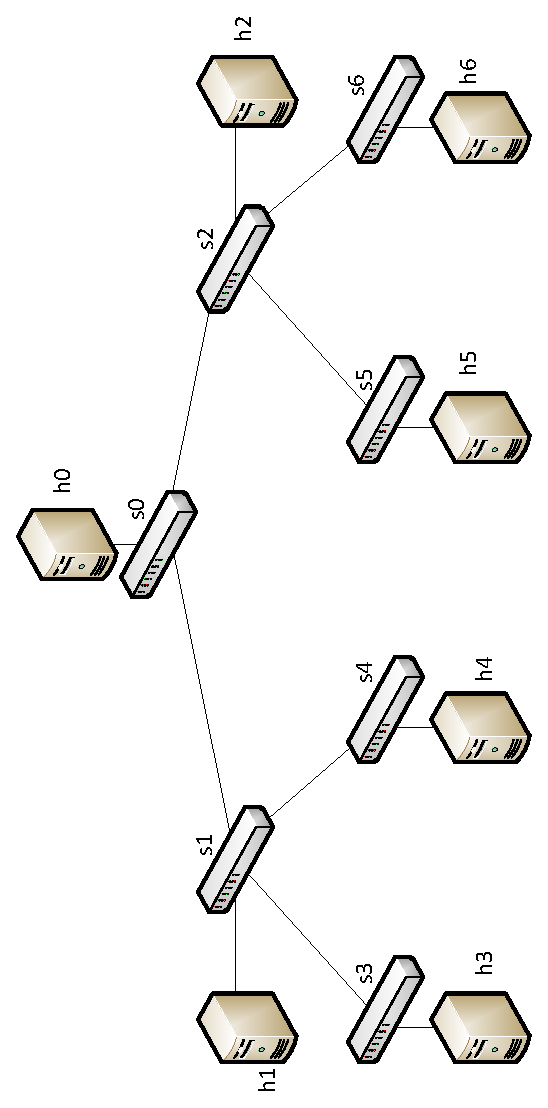
\includegraphics[angle=-90, width=0.48\textwidth, clip]{figs/tree.eps}
}

\caption{Different Network Topologies Considered in This Paper} 
\label{fig:topo}
\end{figure}

To measure the network behaviors, we leverage Mininet \cite{Mininet:official}
to simulate the network with different topologies. In order to make our simulation
close to the real-world network, we need to set certain parameters (\eg network 
delay, packet loss rate) when we construct the topologies. These parameter may be
variable, but for simplicity, we set the same parameter for all network links. 

Our scenario works with one server and multiple clients, each hiding behind a 
switch, as shown in Figure~\ref{fig:topo}.

In theory, at least 3 hops are required for any host to reach another host according
to Figure~\ref{fig:topo}. Then ideally, it is the optimal structure to place the server 
at a location where all clients need only 3 hops to reach it. As we can see, only 
when the server is placed at the center ({\it h0}) in star topology, the optimal 
structure satisfies. This will be verified in our evaluation.

Because every network topology contains multiple nodes that hold a host and every 
host can be used as a server, we need to measure the network for all potential servers
and discover the best location for placing the server in each topology and for all
topologies considered. Due to the symmetry nature of the networks, 4 hosts in line topology
need to be simulated as the server separately, {\it h0}, {\it h1}, {\it h2} and 
{\it h3}; 3 hosts for tree topology, {\it h0}, {\it h1} and {\it h3}; and 
2 hosts for star topology, {\it h0} and anyone else (\eg {\it h1}). 

With the same network parameters, the distance seems to be the only factor that 
influences the throughput. 
Table~\ref{table:distance} depicts the average distance to 
a selected server in network topology. Column 3 shows the local rank
of the average distances in a specific topology and the last 
column presents the global rank of the distances among all 
potential servers in all topologies. 
Ideally, if we only take the distance into account, 
we can infer that the best locations for the server should be {\it h0} 
in star topology, {\it h0} in tree topology, {\it h1} in star topology and 
{\it h1} in tree topology while the last two have the same average distance
to the other nodes. The worst ones should be {\it h0}, {\it h1} in line topology, 
and {\it h3} in tree topology.

\begin{table}[ht]
\centering
	\caption{Average Distance to Selected Servers}
	\label{table:distance}
	\begin{tabular}{|l||c|c|c|}
		\hline 
		Server   &  Avg. Distance & Local Rank & Global Rank \\ \hline\hline
		Line-h0  &   5.50  &  4   &  9 \\ \hline 
		Line-h1  &   4.67  &  3   &  7 \\ \hline 
		Line-h2  &   4.17  &  2   &  6 \\ \hline 
		Line-h3  &   4.00  &  1   &  5 \\ \hline\hline 
		Star-h0  &   3.00  &  1   &  1 \\ \hline 
        Star-h1  &   3.83  &  2   &  3 \\ \hline\hline 
		Tree-h0  &   3.67  &  1   &  2 \\ \hline 
		Tree-h1  &   3.83  &  2   &  3 \\ \hline 
		Tree-h3  &   4.67  &  3   &  7 \\ \hline 
	\end{tabular}
\end{table}

In Mininet, we sequentially choose the hosts mentioned above 
to act the server and all other hosts act as clients. All clients transmit
data packets to the server and the server measures the throughput for all 
incoming connections. By this means, we can measure the performance of 
all potential servers. 